% Template file for an a0 landscape poster.
% Written by Graeme, 2001-03 based on Norman's original microlensing
% poster.
%
% See discussion and documentation at
% <http://www.astro.gla.ac.uk/users/norman/docs/posters/> 
%
% $Id: poster-template-landscape.tex,v 1.2 2002/12/03 11:25:46 norman Exp $


% Default mode is landscape, which is what we want, however dvips and
% a0poster do not quite do the right thing, so we end up with text in
% landscape style (wide and short) down a portrait page (narrow and
% long). Printing this onto the a0 printer chops the right hand edge.
% However, 'psnup' can save the day, reorienting the text so that the
% poster prints lengthways down an a0 portrait bounding box.
%
% 'psnup -w85cm -h119cm -f poster_from_dvips.ps poster_in_landscape.ps'

\documentclass[a0]{a0poster}
% You might find the 'draft' option to a0 poster useful if you have
% lots of graphics, because they can take some time to process and
% display. (\documentclass[a0,draft]{a0poster})
\input defs
\pagestyle{empty}
\setcounter{secnumdepth}{0}
\renewcommand{\familydefault}{\sfdefault}
\newcommand{\QED}{~~\rule[-1pt]{8pt}{8pt}}\def\qed{\QED}

\renewcommand{\reals}{{\mbox{\bf R}}}

% The textpos package is necessary to position textblocks at arbitary 
% places on the page.
\usepackage[absolute]{textpos}

\usepackage{fleqn,psfrag,wrapfig,tikz}

\usepackage[papersize={38in,28in}]{geometry}

% Graphics to include graphics. Times is nice on posters, but you
% might want to switch it off and go for CMR fonts.
% \usepackage{graphics}


\usepackage{hyperref}


% we are running pdflatex, so convert .eps files to .pdf
\usepackage{graphicx}
\usepackage[font=small,labelfont=bf]{caption}
\graphicspath{ {images/} }
%\usepackage{epstopdf}

% These colours are tried and tested for titles and headers. Don't
% over use color!
\usepackage{color}
\definecolor{Red}{rgb}{0.9,0.0,0.1}

\definecolor{bluegray}{rgb}{0.15,0.20,0.40}
\definecolor{bluegraylight}{rgb}{0.35,0.40,0.60}
\definecolor{gray}{rgb}{0.3,0.3,0.3}
\definecolor{lightgray}{rgb}{0.7,0.7,0.7}
\definecolor{darkblue}{rgb}{0.2,0.2,1.0}
\definecolor{darkgreen}{rgb}{0.0,0.5,0.3}

\renewcommand{\labelitemi}{\textcolor{bluegray}\textbullet}
\renewcommand{\labelitemii}{\textcolor{bluegray}{--}}

\setlength{\labelsep}{0.5em}


% see documentation for a0poster class for the size options here
\let\Textsize\normalsize
%\def\Head#1{\noindent\hbox to \hsize{\hfil{\LARGE\color{bluegray} #1}}\bigskip}
\def\Head#1{\noindent{\LARGE\color{bluegray} #1}\bigskip}
\def\LHead#1{\noindent{\LARGE\color{bluegray} #1}\bigskip}
\def\Subhead#1{\noindent{\large\color{bluegray} #1}\bigskip}
\def\Title#1{\noindent{\VeryHuge\color{Red} #1}}


% Set up the grid
%
% Note that [40mm,40mm] is the margin round the edge of the page --
% it is _not_ the grid size. That is always defined as 
% PAGE_WIDTH/HGRID and PAGE_HEIGHT/VGRID. In this case we use
% 23 x 12. This gives us three columns of width 7 boxes, with a gap of
% width 1 in between them. 12 vertical boxes is a good number to work
% with.
%
% Note however that texblocks can be positioned fractionally as well,
% so really any convenient grid size can be used.
%
\TPGrid[40mm,40mm]{23}{12}      % 3 cols of width 7, plus 2 gaps width 1

\parindent=0pt
\parskip=0.2\baselineskip

\begin{document}

% Understanding textblocks is the key to being able to do a poster in
% LaTeX. In
%
%    \begin{textblock}{wid}(x,y)
%    ...
%    \end{textblock}
%
% the first argument gives the block width in units of the grid
% cells specified above in \TPGrid; the second gives the (x,y)
% position on the grid, with the y axis pointing down.

% You will have to do a lot of previewing to get everything in the 
% right place.

% This gives good title positioning for a portrait poster.
% Watch out for hyphenation in titles - LaTeX will do it
% but it looks awful.
\begin{textblock}{23}(0,0)
\Title{Deep Learning for Segmentation and Counting within Microscopy Data}
\end{textblock}

\begin{textblock}{23}(0,0.6)
{
\LARGE
\vspace{5mm}
Carlos Xavier Hern\'{a}ndez and Mohammad Muneeb Sultan
}

{
\Large
\color{bluegray}
\vspace{5mm}
\emph{CS231N: Convolutional Neural Networks for Visual Recognition Class Project}
}
\end{textblock}


% Uni logo in the top right corner. A&A in the bottom left. Gives a
% good visual balance, but you may want to change this depending upon
% the graphics that are in your poster.
%\begin{textblock}{2}(0,10)
%Your logo here
%%\includegraphics{/usr/local/share/images/AandA.epsf}
%\end{textblock}

%\begin{textblock}{2}(21.2,0)
%Another logo here
%%\resizebox{2\TPHorizModule}{!}{\includegraphics{/usr/local/share/images/GUVIu/GUVIu.eps}}
%\end{textblock}


\begin{textblock}{7.0}(0,1.5)

\hrule\medskip
\Head{Motivation}\\
Cell counting is a ubiquitous, yet tedious task that would greatly benefit from automation.
From basic biological questions to clinical trials, cell counts provide key quantitative
feedback that drive research. Unfortunately, cell counting is most commonly a manual task
and can be time-intensive. The task is also made more difficult due to overlapping cells,
existence of multiple focal planes, and poor imaging quality, among other things.
Here, we attempt to automate both the segmentation and counting of cells for a given
microscopy image. We hope to create a useful tool for biologist and ultimately expedite research.

\medskip
\hrule\medskip
\Head{Previous Work}\\
At the moment there is no state-of-the-art convolutional neural network (CNN) architecture for
counting objects in an image, much less counting cells. However, there is quite a bit of ongoing
research in the field of image segmentation using CNNs on which we based our methodology:

\begin{itemize}\itemsep=12pt
\item Mask R-CNN (\href{https://arxiv.org/abs/1703.06870}{arXiv:1703.06870})
\item Feature Pyramid Networks (\href{https://arxiv.org/abs/1612.03144}{arXiv:1612.03144})
\item Uncertainty in Bayesian Deep Learning for Computer Vision (\href{https://arxiv.org/abs/1703.04977}{arXiv:1703.04977})
\end{itemize}

There has also been previous work done in the task of segmenting and classifying cell types using CNNs:

\begin{itemize}\itemsep=12pt
\item DeepCell (\href{https://doi.org/10.1371/journal.pcbi.1005177}{10.1371/journal.pcbi.1005177})
\end{itemize}

\medskip
\hrule\medskip
\Head{Dataset}\\
We used the \href{https://data.broadinstitute.org/bbbc/BBBC005/}{BBBC005 dataset} from the
Broad Institute's Bioimage Benchmark Collection. This dataset is a collection of 9,600 simulated microscopy
images of stained cells. These images were simulated for a given cell count with a clustering probability
of 25\%. Focus blur was simulated by applying Gaussian filters to the images. Each image is 696 x 520
pixels in 8-bit TIFF format (eventually converted to JPEG and scaled down to 256 x 192 pixels),
with cell areas matched to the average cell areas of human U2OS cells.
Of the 9,600 images, 600 images have a corresponding foreground mask.


For each experiment, we used an 80/20 split for training and validation.

\medskip
\hrule\medskip
\Head{Cell Segmentation}\\
\vspace{-1.5cm}
\begin{figure}[!h]
\centering
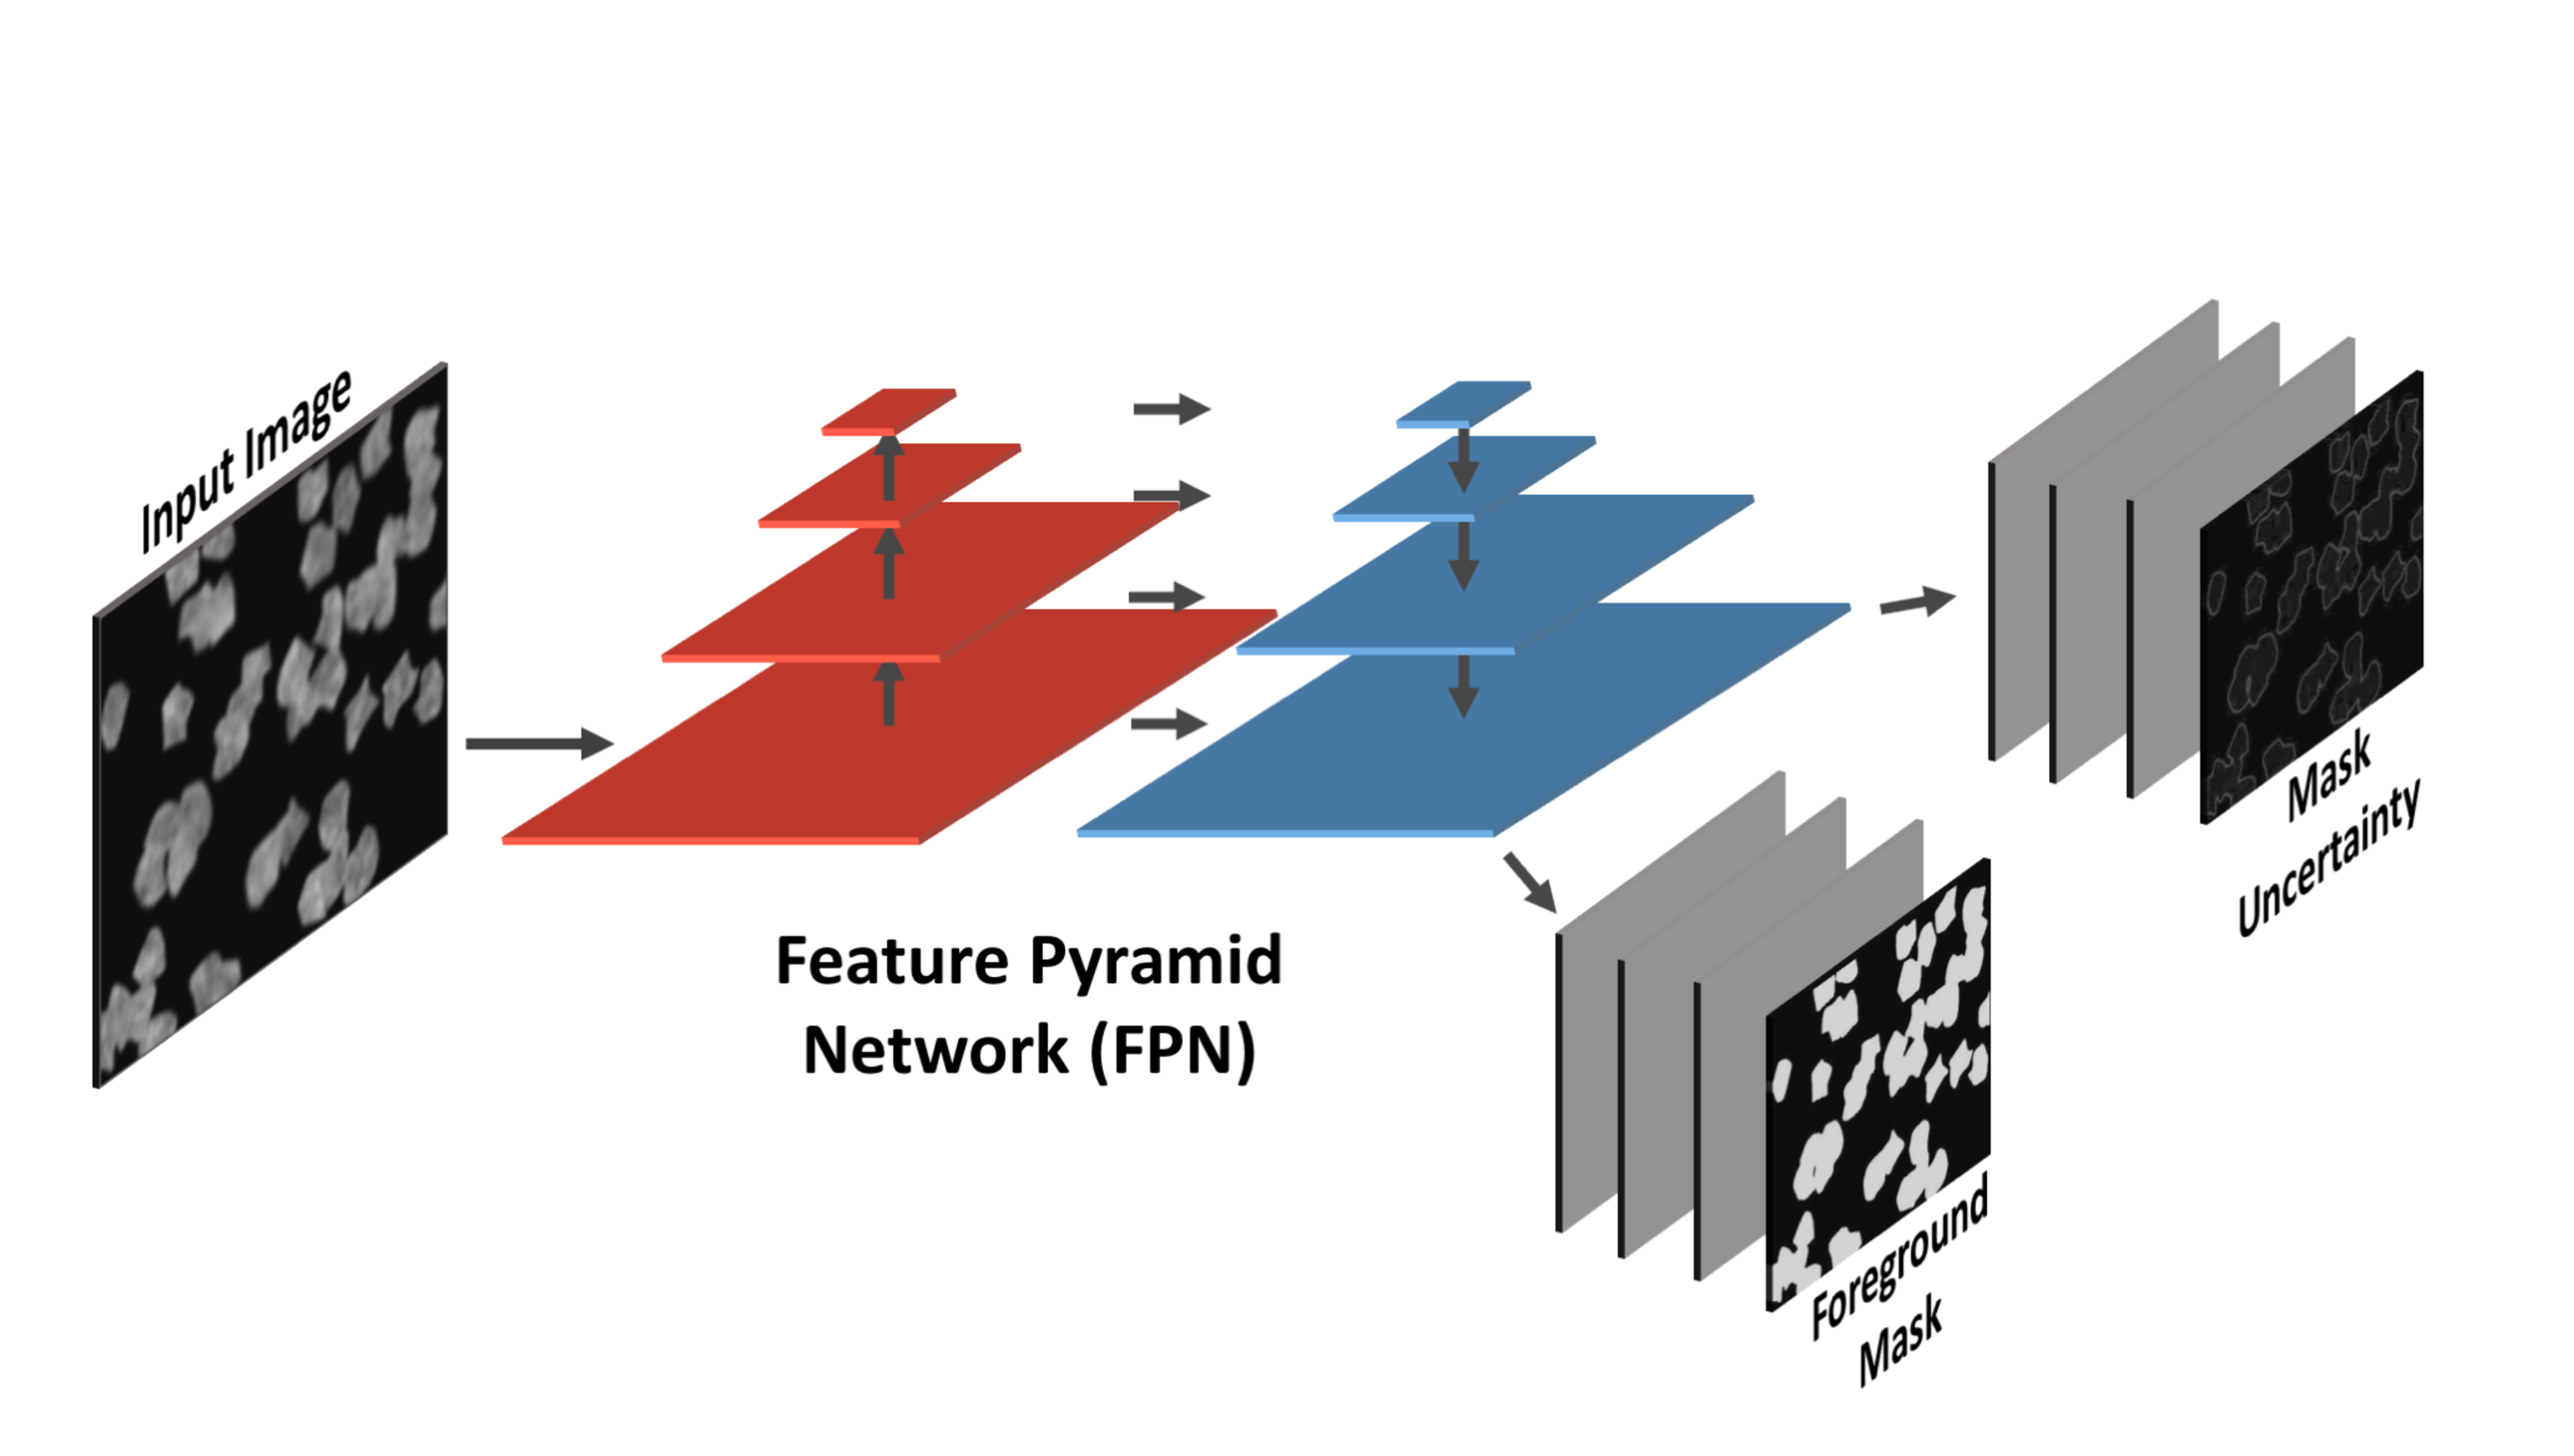
\includegraphics[width=0.9\textwidth]{fpn}
\caption{A schematic of our Feature Pyramid Network for generating a foreground mask.}
\end{figure}

\end{textblock}

\begin{textblock}{7.0}(8,1.5)
\hrule\medskip
\Head{Cell Counting}\\
\vspace{-1.5cm}
\begin{figure}[!h]
\centering
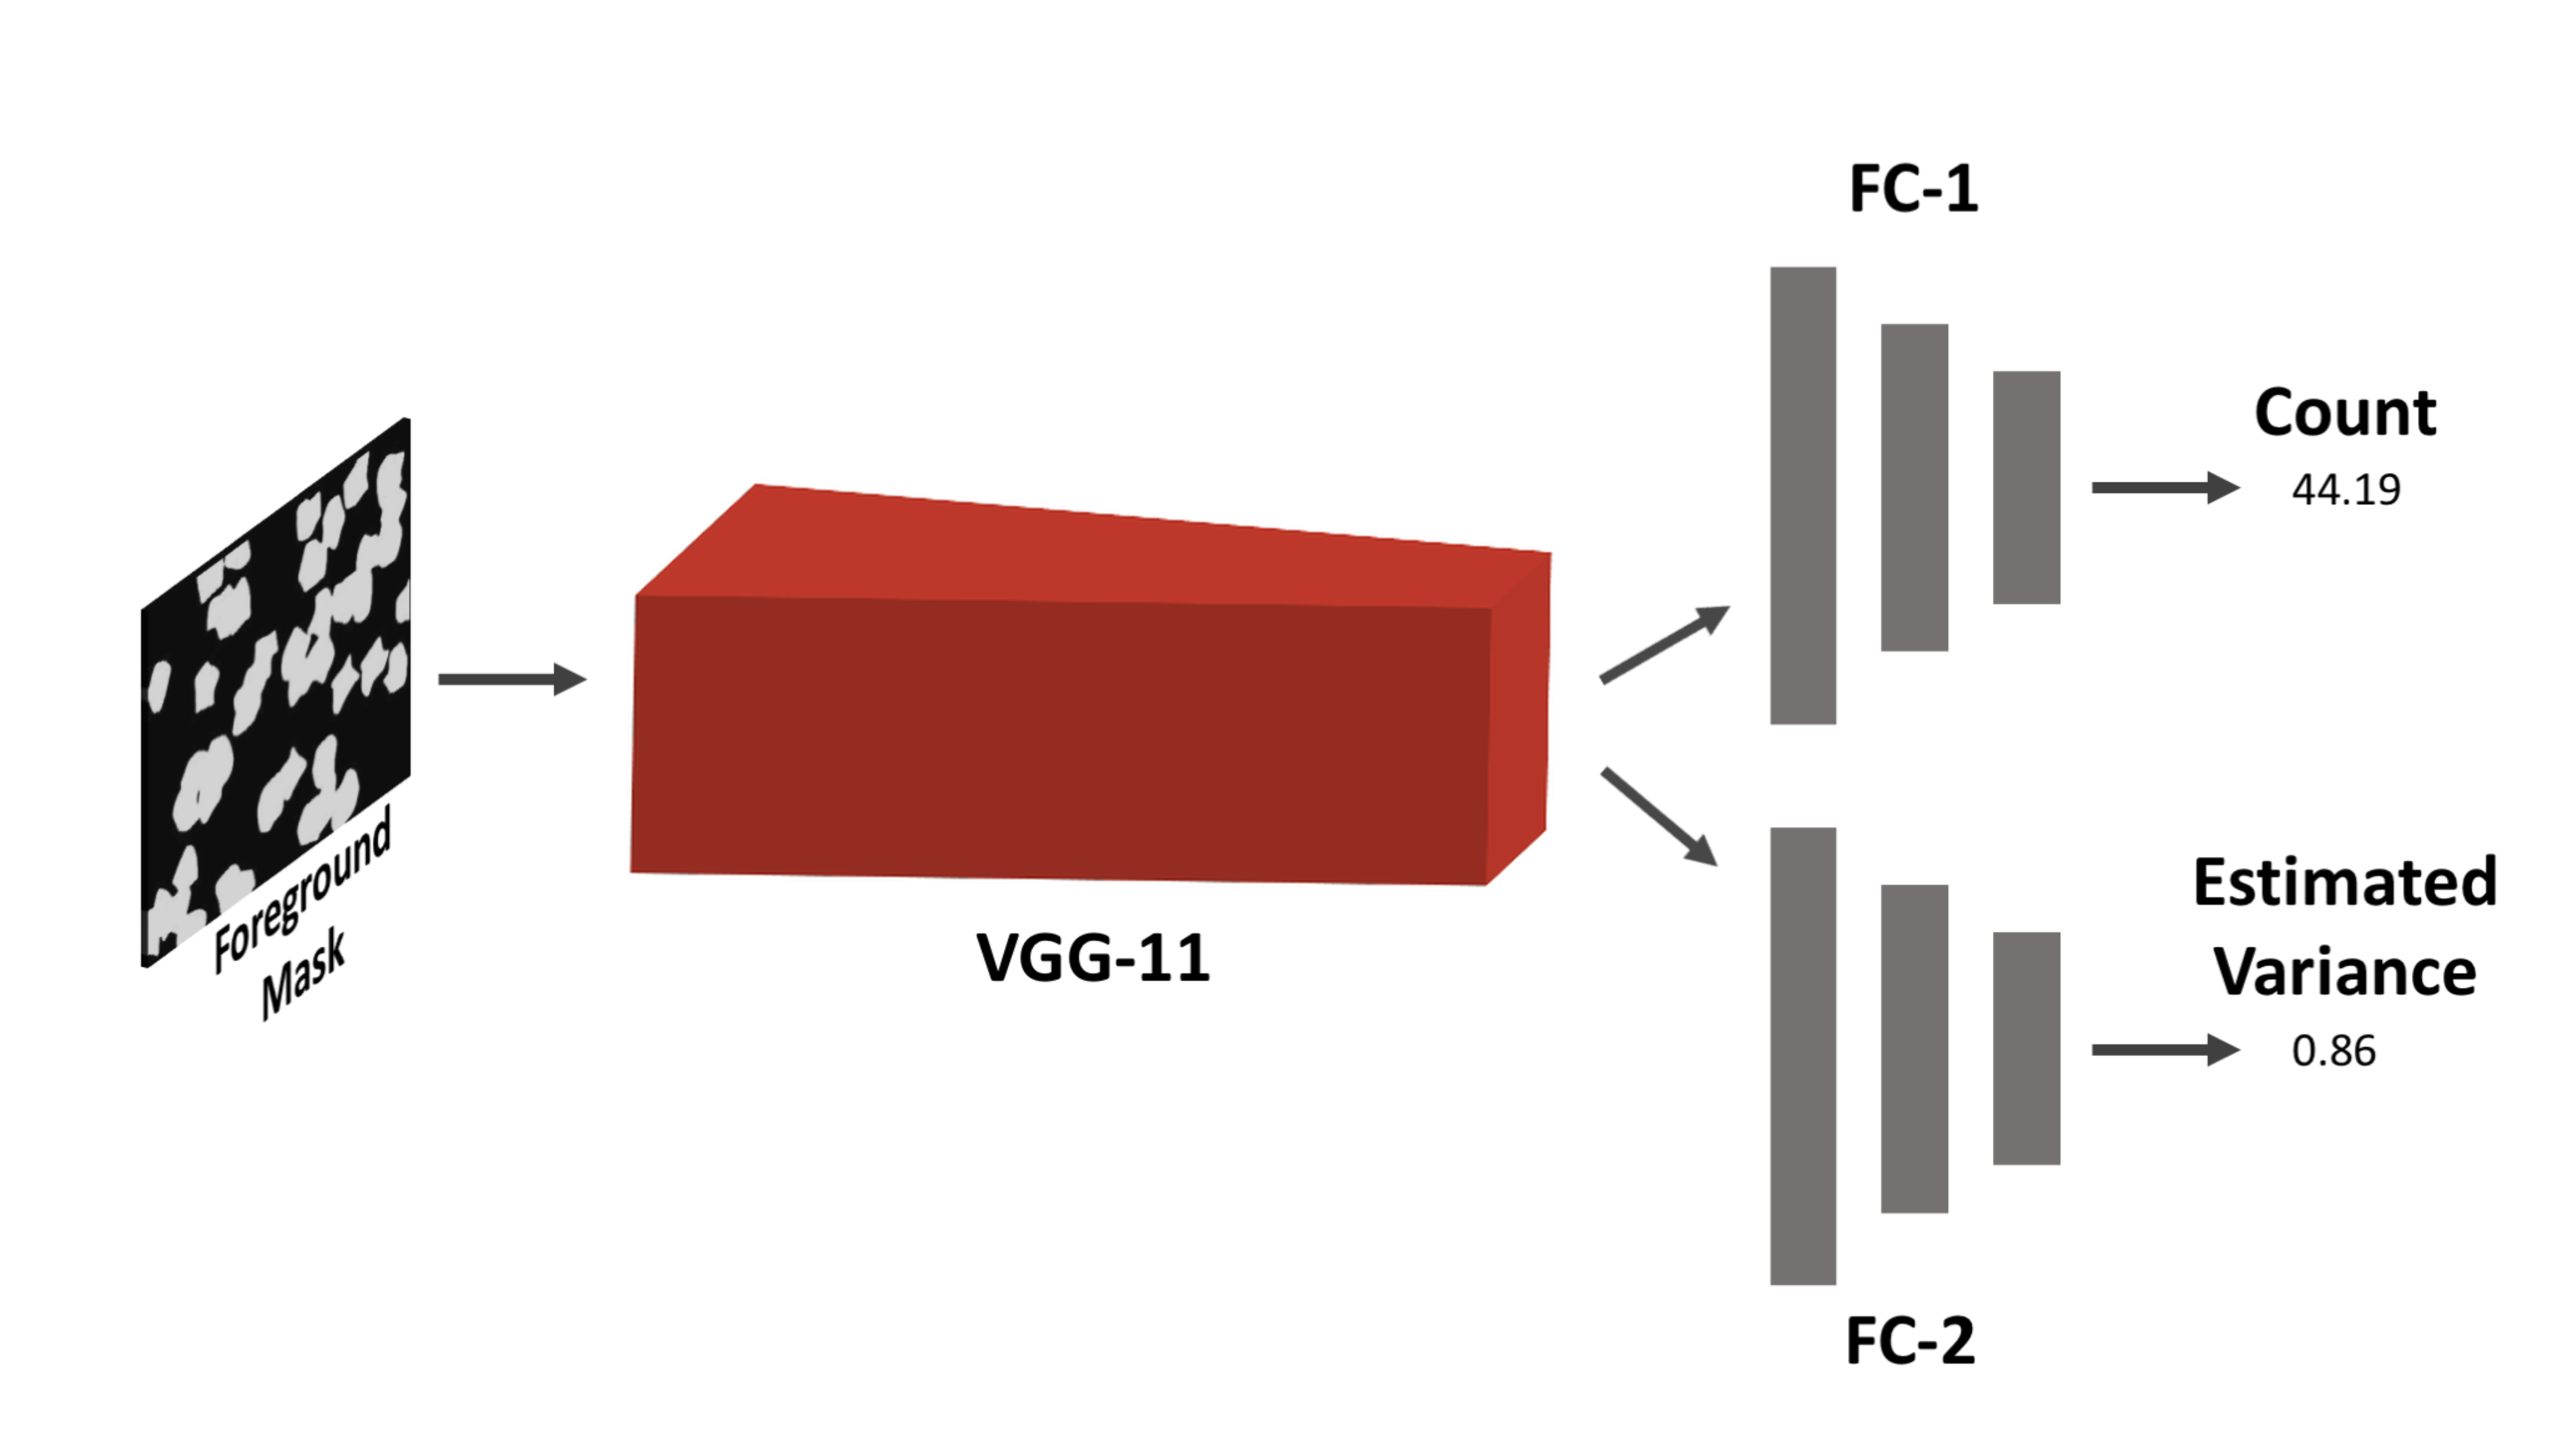
\includegraphics[width=0.9\textwidth]{count}
\caption{A schematic of our VGG-11-based network for counting cells from a foreground mask.}
\end{figure}

\medskip
\hrule\medskip
\Head{Experiments}\\
Pre-trained FPN on 480 images with known foregrounds:
\begin{itemize}\itemsep=12pt
\item Backprop on L1 (w/ aleatoric uncertainty) and TV losses for each output mask using ADAM optimizer
\item Converged validation MSE on 120 validation images after 50 epochs
\end{itemize}

Trained VGG-11-based network on 7,680 FPN-generated masks:
\begin{itemize}\itemsep=12pt
\item Backprop on L1 (w/ aleatoric uncertainty) loss with cell counts using ADAM optimizer
\item Converged validation MSE between counts on 1,920 validation images after 50 epochs
\end{itemize}

\medskip
\hrule\medskip
\Head{Results}\\
After 50 epochs of training, our best model is able to achieve an $R^2$ value of .987.
80\% of the time, the ground truth falls within the predicted 95\% confidence interval.

\vspace{5mm}
\begin{figure}[!h]
\centering
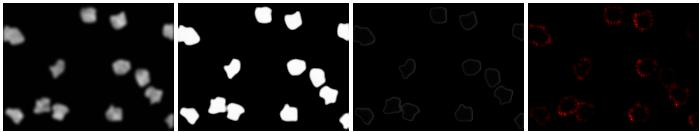
\includegraphics[width=0.95\textwidth]{good-1}
\caption{A validation example from our model with 14 cells.
The left-most sub-figure is the input image to our model.
To its right is the predicted foreground mask for the input and its associated uncertainty, respectively.
The right-most sub-figure depicts the saliency map during counting.
Our model predicts that this image has 14.00 $\pm$ 1.82 number of cells with 95\% confidence.}
\end{figure}
\vspace{5mm}
\begin{figure}[!h]
\centering
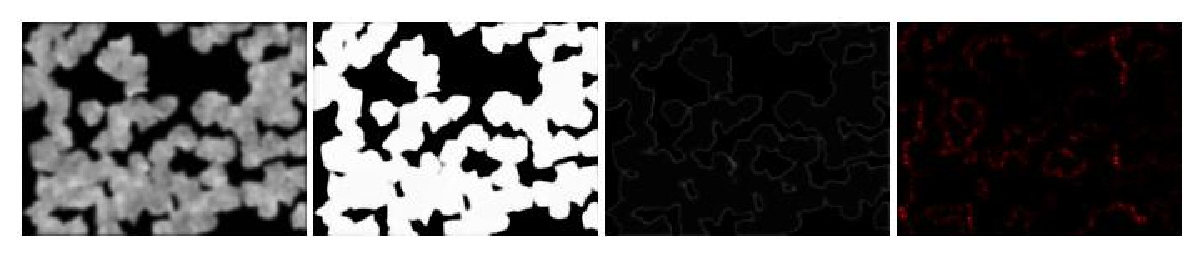
\includegraphics[width=0.95\textwidth]{good-2}
\caption{Model thinks this image has 96.17 $\pm$ 3.62 cells. Ground truth is 96 cells.}
\end{figure}

\end{textblock}

\begin{textblock}{7.0}(16,1.5)

\hrule\medskip
\Head{Failure Cases}\\
We find that our method systematically fails in a number of cases:

\begin{itemize}\itemsep=12pt
\item Lots of Overlapping Cells

\begin{figure}[!h]
\centering
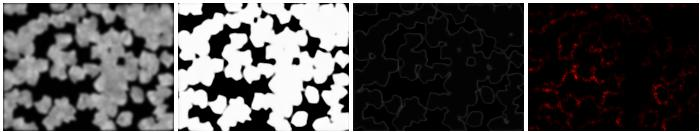
\includegraphics[width=0.95\textwidth]{bad-1}
\caption{Model thinks this image has 93.50 $\pm$ 3.51 cells. Ground truth is 100 cells.}
\end{figure}


\item Oddly Shaped Cells

\begin{figure}[!h]
\centering
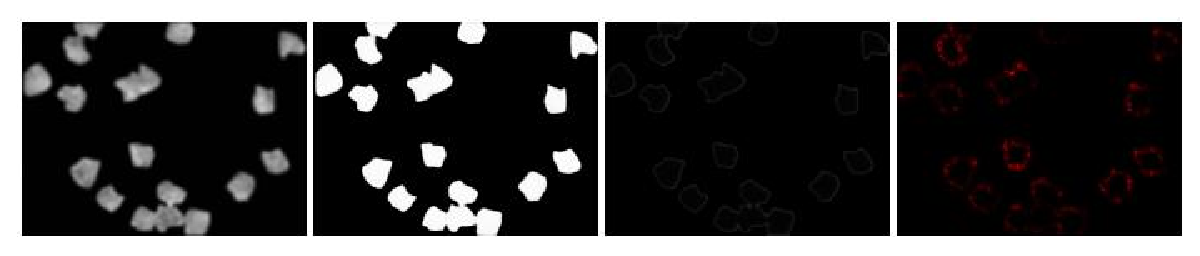
\includegraphics[width=0.95\textwidth]{bad-2}
\caption{Model thinks this image has 22.83 $\pm$ 2.19 cells. Ground truth is 18 cells.}
\end{figure}


\item Bad Focal Planes

\begin{figure}[!h]
\centering

\includegraphics[width=0.95\textwidth]{bad-3}
\caption{Model thinks this image has 11.85 $\pm$ 1.77 cells. Ground truth is 14 cells.}
\end{figure}

\end{itemize}

\medskip
\hrule\medskip
\Head{Conclusion}\\
We show that it is possible to design and train a CNN architecture to count cells in microscopy images
with relatively good accuracy. While there are a number of failures cases that arise, we believe that
better training data might help to overcome these. Specifically, the dataset used lacked foreground masks
for out-of-focus images, which could have helped greatly in improving performance.

We also demonstrate a good use-case for aleatoric losses in estimating uncertainty
in cell counting. As the eventual goal is to create a scientific tool, generating error bounds is
essential, as it improves the statistical power of our method and yields the ability to form
better informed hypotheses.

\medskip
\hrule\medskip
\Head{Acknowledgements}\\
We would like to thank Bharath Ramsundar and Timnit Gebru for helpful conversations and feedback.

All code (as well as this poster and a manuscript) will be made publicly available on GitHub
(\href{https://github.com/cxhernandez/cellcount}{https://github.com/cxhernandez/cellcount}).

\end{textblock}

\end{document}
